% Main editable report. Compile with LuaLaTeX or XeLaTeX, not pdfLaTeX.
% Build from the project root: python report/build_snapshot.py --wsl Debian
\documentclass[12pt,a4paper]{article}
% Shared formatting: edit this file to change the whole report.
% Required: A4; 25 mm margins; Times New Roman 12 pt; 1.5 body spacing.
\usepackage[margin=25mm,headheight=14pt,headsep=7mm,footskip=12mm]{geometry}
\usepackage{fontspec}
\IfFontExistsTF{Times New Roman}{
  \setmainfont{Times New Roman}
}{
  \setmainfont{times.ttf}[
    Path=/mnt/c/Windows/Fonts/,
    BoldFont=timesbd.ttf,
    ItalicFont=timesi.ttf,
    BoldItalicFont=timesbi.ttf
  ]
}
\IfFontExistsTF{Courier New}{
  \setmonofont{Courier New}
}{
  \setmonofont{cour.ttf}[
    Path=/mnt/c/Windows/Fonts/,
    BoldFont=courbd.ttf,
    ItalicFont=couri.ttf,
    BoldItalicFont=courbi.ttf
  ]
}
\usepackage{setspace}
\onehalfspacing
\usepackage{microtype}
\usepackage{graphicx}
\usepackage{pdfpages}
\usepackage{pdflscape}
\usepackage{amsmath,amssymb}
\usepackage{array,tabularx,booktabs}
\usepackage{longtable}
\usepackage{color}
\usepackage{caption}
\usepackage{listings}
\usepackage{fancyhdr}
\usepackage[unicode,hidelinks]{hyperref}
\usepackage{bookmark}

\definecolor{inkblue}{RGB}{35,57,78}
\definecolor{rulegray}{RGB}{164,173,182}
\definecolor{codegray}{RGB}{247,248,250}
\definecolor{commentgreen}{RGB}{57,100,79}
\definecolor{stringred}{RGB}{142,62,53}
\definecolor{numbergray}{RGB}{93,105,116}
\hypersetup{
  pdftitle={Fortune's Sweep-Line Algorithm for Planar Voronoi Diagrams},
  pdfauthor={Mineth Lohiru Ariyarathna},
  pdfsubject={Implementation, validation and AI-assisted development},
  pdfkeywords={Fortune algorithm, Voronoi diagram, computational geometry}
}
\graphicspath{{figures/}{../figures/}{../evidence/}}
\urlstyle{same}
\DeclareUrlCommand\path{\def\UrlFont{\ttfamily\fontsize{10}{12}\selectfont}}
\Urlmuskip=0mu plus 1mu\relax
\setlength{\parindent}{0pt}
\setlength{\parskip}{5pt}
\setlength{\emergencystretch}{2em}
\setlength{\textfloatsep}{14pt plus 2pt minus 2pt}
\setlength{\intextsep}{12pt plus 2pt minus 2pt}
\setlength{\floatsep}{12pt plus 2pt minus 2pt}
\renewcommand{\topfraction}{0.92}
\renewcommand{\bottomfraction}{0.80}
\renewcommand{\textfraction}{0.07}
\renewcommand{\floatpagefraction}{0.72}
\raggedbottom
\widowpenalty=10000
\clubpenalty=10000
\displaywidowpenalty=10000

\makeatletter
\renewcommand\section{\@startsection{section}{1}{\z@}
  {-2.2ex\@plus -0.8ex\@minus -0.2ex}
  {1.0ex\@plus 0.2ex}{\normalfont\fontsize{15}{19}\selectfont\bfseries}}
\renewcommand\subsection{\@startsection{subsection}{2}{\z@}
  {-1.8ex\@plus -0.5ex\@minus -0.2ex}
  {0.7ex\@plus 0.2ex}{\normalfont\fontsize{12}{18}\selectfont\bfseries}}
\renewcommand{\@seccntformat}[1]{\csname the#1\endcsname.\quad}
\makeatother

\captionsetup{
  font={normalsize},labelfont=bf,labelsep=period,
  justification=raggedright,singlelinecheck=false,skip=6pt
}
\captionsetup[table]{position=top}
\renewcommand{\arraystretch}{1.18}
\setlength{\tabcolsep}{5pt}

\lstdefinestyle{reportcode}{
  language=Python,
  basicstyle=\ttfamily\fontsize{9.5}{12}\selectfont,
  keywordstyle=\color{inkblue}\bfseries,
  commentstyle=\color{commentgreen}\itshape,
  stringstyle=\color{stringred},
  showstringspaces=false,
  breaklines=true,
  columns=fullflexible,
  keepspaces=true,
  numbers=left,
  numberstyle=\ttfamily\fontsize{9}{11}\selectfont\color{numbergray},
  numbersep=9pt,
  xleftmargin=16pt,
  xrightmargin=2pt,
  frame=single,
  framerule=0.3pt,
  rulecolor=\color{rulegray},
  backgroundcolor=\color{codegray},
  framesep=6pt,
  aboveskip=12pt,
  belowskip=12pt,
  lineskip=1pt,
  captionpos=t
}
\lstset{style=reportcode}
\newcommand{\code}[1]{{\ttfamily\fontsize{10}{12}\selectfont #1}}

\newcommand{\ReportPageStyle}{
  \fancyhf{}
  \fancyhead[L]{\fontsize{9}{11}\selectfont Fortune's Sweep-Line Algorithm}
  \fancyhead[R]{\fontsize{9}{11}\selectfont Computational Geometry}
  \fancyfoot[C]{\fontsize{10}{12}\selectfont\thepage}
  \renewcommand{\headrulewidth}{0.3pt}
  \renewcommand{\footrulewidth}{0pt}
}
\fancypagestyle{reportbody}{\ReportPageStyle}
\fancypagestyle{plain}{\ReportPageStyle}
\pagestyle{reportbody}

% Wide, unaltered terminal captures use the full landscape text area.
\newcommand{\EvidenceLandscape}[4]{
  \clearpage
  \begin{landscape}
  \thispagestyle{empty}
  \captionsetup{hypcap=false}
  \centering
  \vspace*{\fill}
  \includegraphics[width=\linewidth,height=132mm,keepaspectratio]{#1}
  \captionof{figure}[#2]{#3}\label{#4}
  \vspace*{\fill}
  {\fontsize{10}{12}\selectfont\thepage\par}
  \end{landscape}
}


\begin{document}
\hypersetup{pageanchor=false}
% The cover is filled in Word using the supplied assignment cover template.
% Import its single-page PDF without adding the former LaTeX cover.
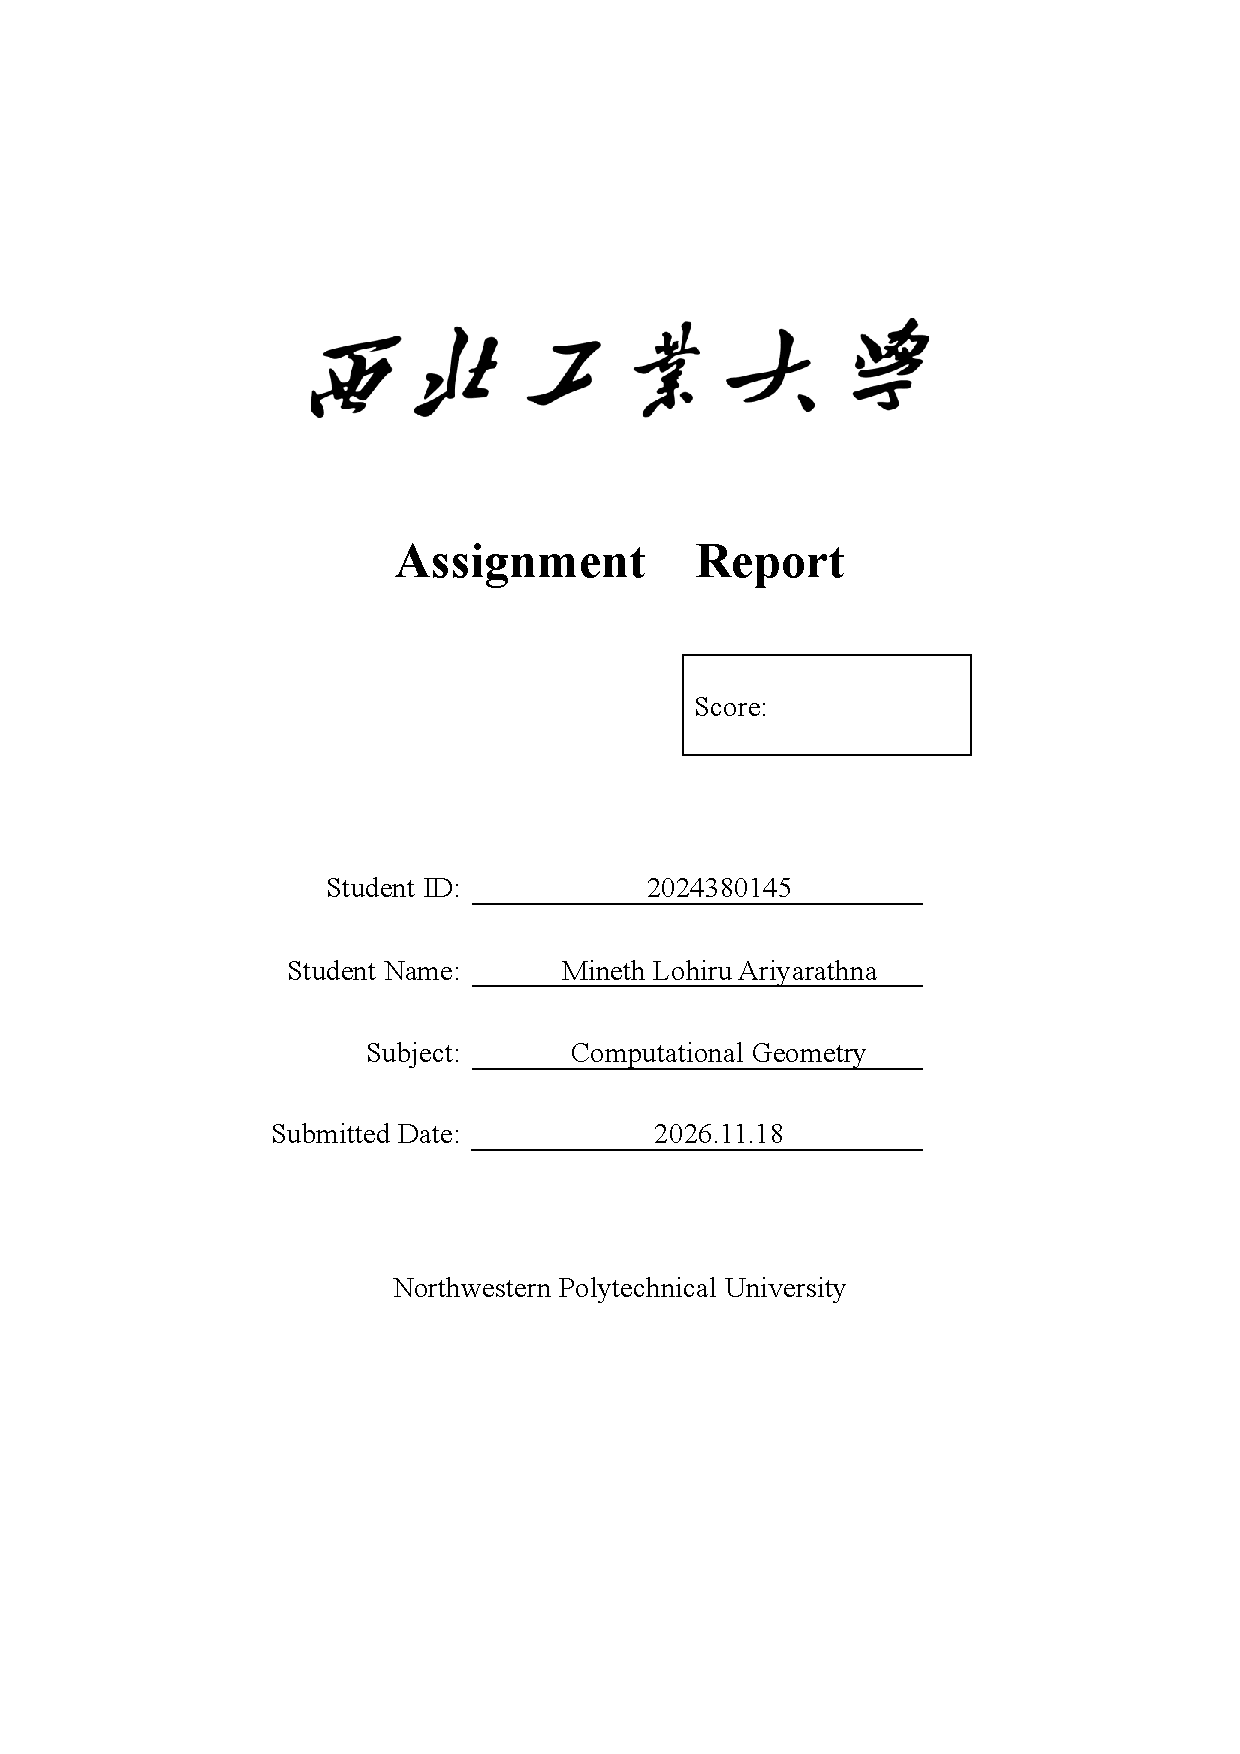
\includepdf[pages=1,pagecommand={\thispagestyle{empty}},fitpaper=true]{cover.pdf}


\pagenumbering{roman}
\hypersetup{pageanchor=true}
\begingroup
\setcounter{tocdepth}{1}
\setstretch{1.05}
\tableofcontents
\endgroup
\vspace{1em}
\noindent\textbf{Companion document.} Appendix A, the complete source listing, is supplied separately as \href{source_appendix.pdf}{\nolinkurl{source_appendix.pdf}}. This volume contains the main report, references and Appendices B--D.
\setcounter{tocdepth}{2}
\clearpage
\begingroup
\setstretch{1.08}
\listoffigures
\vspace{1.5em}
\listoftables
\endgroup
\clearpage

\pagenumbering{arabic}
% Editable report section: Introduction and Theoretical Background
\section{Introduction and Theoretical Background}
\label{sec:1}

The geometric core implements Fortune's sweep-line algorithm to construct planar Voronoi diagrams from point sites. The program maintains a balanced beach line and an event queue, handles circle-event invalidation, and builds ordered cells clipped to a bounding rectangle. Batch commands and a graphical point-entry interface provide image and machine-readable exports. A 171-test suite, independent geometric checks and a separate reference comparison check the output. The program also provides an event replay and a Delaunay overlay. This report covers the implementation and verification available on 18 November 2026; the current construction benchmark was measured on the same date, with earlier measurements retained separately. The finite-precision limits of the implementation remain important when interpreting those results.

For sites \(P=\{p_1,\ldots,p_n\}\subset\mathbb{R}^2\), the Voronoi cell of \(p_i\) contains each query \(q\) at least as close to \(p_i\) as to every other site:
\begin{equation}
  V_i=\left\{q\in\mathbb{R}^2:
  \lVert q-p_i\rVert_2\leq\lVert q-p_j\rVert_2
  \quad\text{for every }j\neq i\right\}.
  \label{eq:cell}
\end{equation}
Each comparison defines a half-plane bounded by a perpendicular bisector. Their intersection is convex and may be unbounded. A clipping rectangle makes its visible portion finite without changing ownership inside that rectangle. Sites on the boundary of the convex hull have unbounded cells; sites strictly inside the hull have bounded cells.

The straight-line dual connects two sites when their Voronoi cells share an edge of positive length. In general position, this gives the Delaunay triangulation. A finite Voronoi vertex is the centre of an empty circumcircle through the sites of its dual triangle. Four or more cocircular sites create a higher-degree Voronoi vertex, so a triangulation of the corresponding Delaunay face is not unique. This distinction matters when choosing which adjacencies represent real Voronoi edges and which are zero-length diagonals.

\begin{figure}[!htbp]
\centering
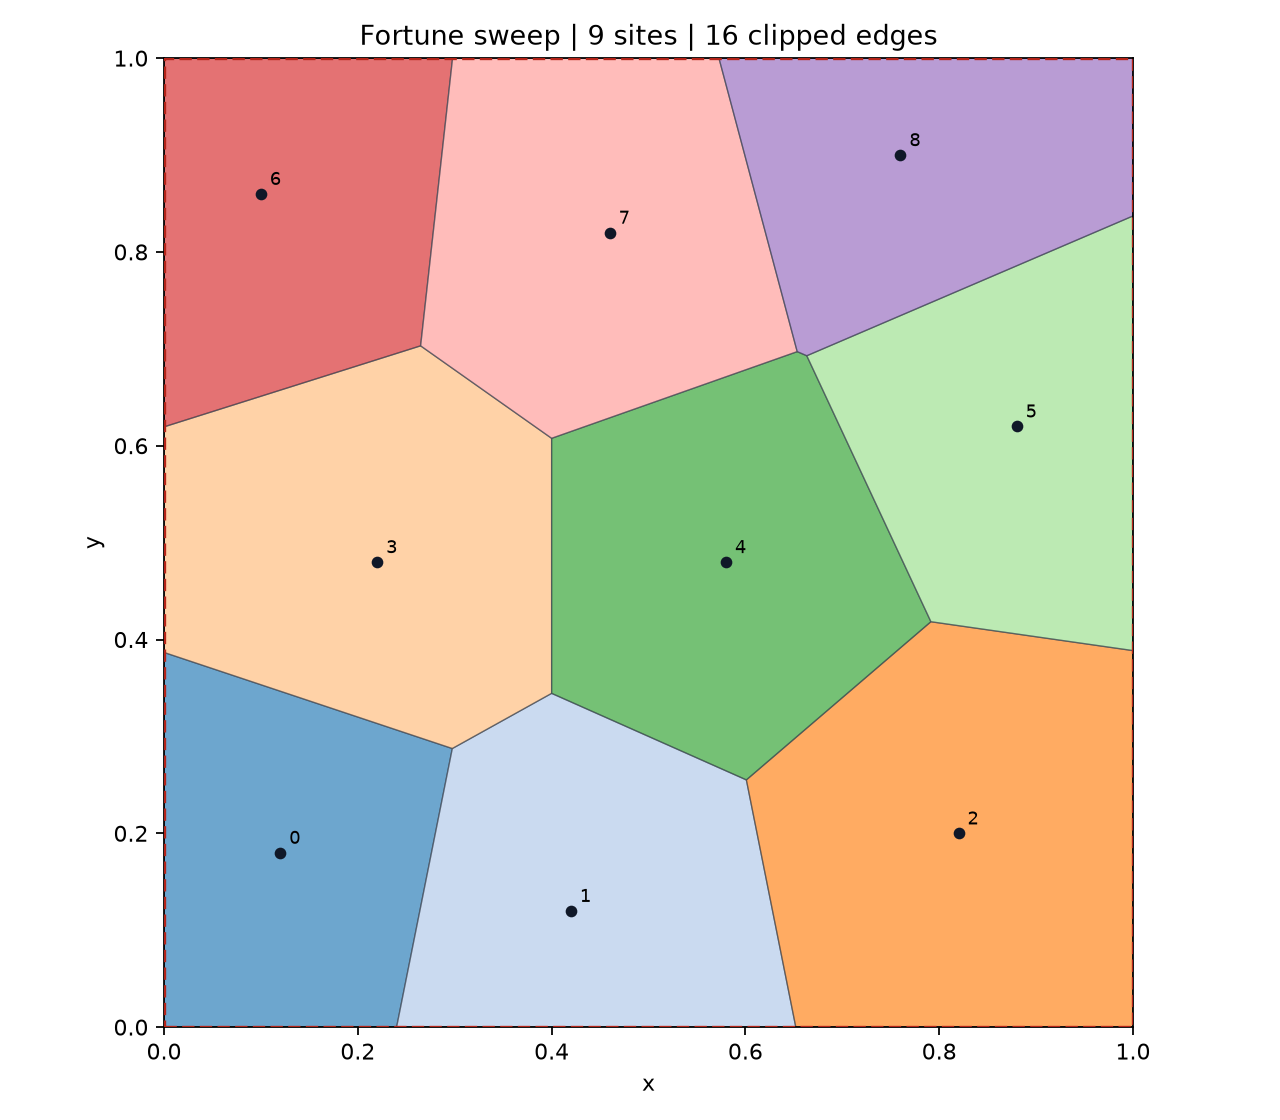
\includegraphics[width=0.86\linewidth,height=0.51\textheight,keepaspectratio]{general.png}
\caption{Nine-site Voronoi diagram clipped to the unit square.}
\label{fig:1}
\end{figure}

The dashed red rectangle is the clipping boundary. Markers and original input indices identify the sites. Shared polygon boundaries represent equal distances. The program distinguishes true circle-event vertices from corners introduced only by clipping.

\subsection{Sweep Mechanics and Degeneracies}

The directrix \(y=\ell\) moves downwards. A processed site \(p=(p_x,p_y)\), with \(p_y>\ell\), and the directrix define the parabola
\begin{equation}
  y=\frac{(x-p_x)^2}{2(p_y-\ell)}+\frac{p_y+\ell}{2}.
  \label{eq:parabola}
\end{equation}
The beach line is the lower envelope of these parabolas. Figure~\ref{fig:2} illustrates this geometric model, rather than an animation frame captured from the implementation.

\begin{figure}[!htbp]
\centering
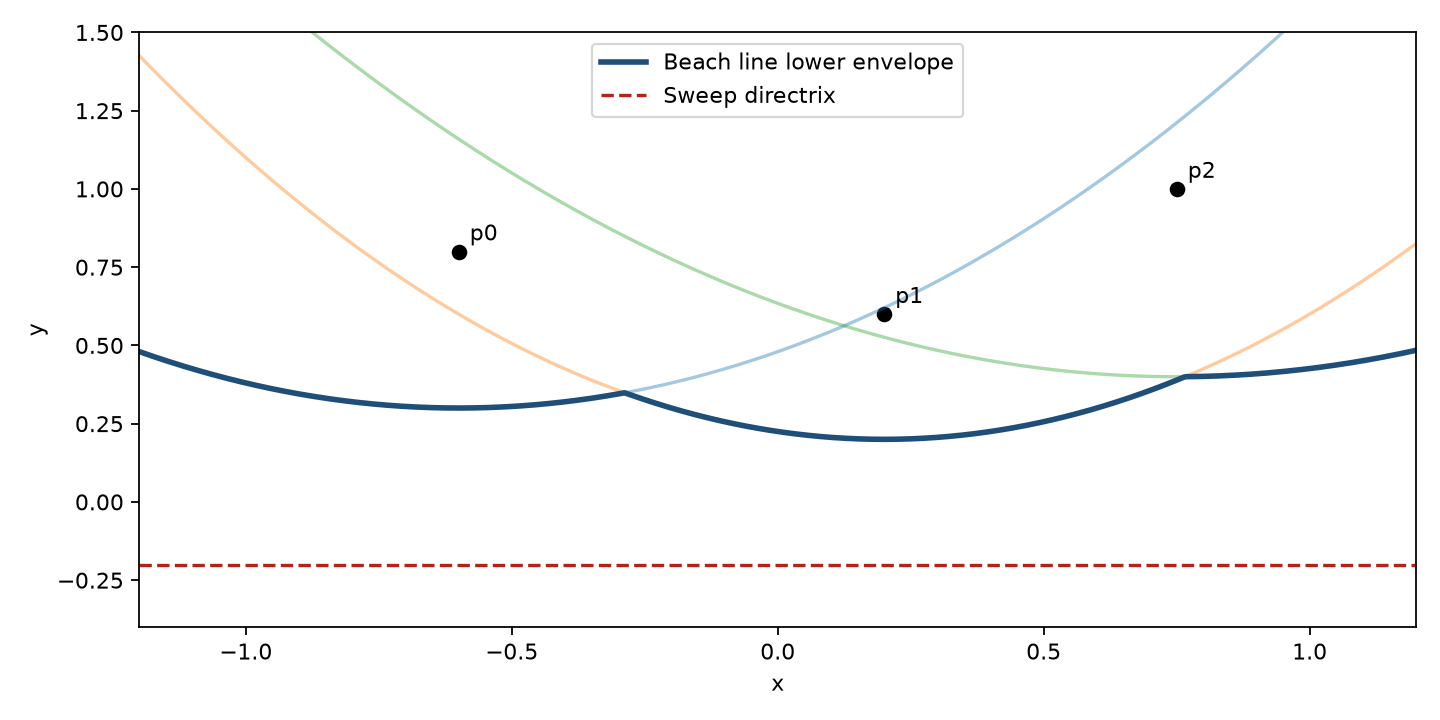
\includegraphics[width=1.0\linewidth,height=0.38\textheight,keepaspectratio]{beachline.png}
\caption{Site parabolas, sweep directrix and the beach-line lower envelope.}
\label{fig:2}
\end{figure}

A site event inserts a limiting arc and normally splits an existing arc into three. At a circle event, three consecutive arcs meet an empty circle and the middle arc disappears. For centre \(c=(c_x,c_y)\) and radius \(r\), the Voronoi vertex is \(c\), while the event height is
\begin{equation}
  \ell_{\mathrm{event}}=c_y-r.
  \label{eq:circle-event}
\end{equation}
Changes to neighbouring arcs can invalidate a pending event before it reaches the front of the queue.

Fortune's original work establishes the sweep approach and its $O(n \log n)$ time and $O(n)$ space bounds \cite{fortune1987}. The core follows the beach-line formulation and uses Python containers and mathematics. Existing Voronoi and Delaunay implementations are not used to construct the diagram.

Degeneracies need explicit policies. Exact duplicates share one cell and retain all original indices. Exactly collinear inputs reduce to consecutive one-dimensional neighbours and parallel bisectors. Equal-height events use limiting arcs. Cocircular events may share one emitted vertex. Near-coincident sites remain distinct, subject to finite-precision representation; no blanket distance threshold silently merges them.

% Editable report section: AI Tools and Development Methodology
\section{AI Tools and Development Methodology}
\label{sec:2}

I used ChatGPT/Codex with GPT-6.1 on ChatGPT Plus, together with Pi 0.86.0 using GPT-6.1 through the OpenAI Codex provider. AI support for the program covered specification extraction, architecture, implementation, tests and measurements. Work progressed from geometric primitives to the AVL beach line, event handling, cell construction and the interfaces, with checks at each stage.

The architecture followed the operations each component needed to support. The beach line needed ordered search, insertion and deletion; the event queue needed deterministic priority and a way to reject obsolete circle events. These requirements provided concrete criteria for assessing a proposed design before integrating its components.

\begin{table}[!htbp]
\centering
\caption{Checks used during AI-assisted implementation.}
\label{tab:1}
\begin{tabularx}{\linewidth}{@{}p{0.34\linewidth}X@{}}
\toprule
\textbf{Development activity} & \textbf{Verification used} \\
\midrule
Geometry and circle construction & Singular-limit, translation and equidistance tests \\
AVL beach line & Random insertion/deletion with structural invariants \\
Sweep and cells & Ownership, area and empty-circle checks \\
Interfaces and replay & CLI exports, callbacks, event stepping and pointer controls \\
Reference comparison & SciPy/Qhull and separate exact all-pairs clipping \\
Performance & Repeated construction timing and isolated memory processes \\
\bottomrule
\end{tabularx}
\end{table}

Figure~\ref{fig:ai-chatgpt} records a ChatGPT explanation of AVL order and generation-based circle-event rejection. The explanation was checked against the arc links, rotations and event guard. Pi also produced four regression tests covering stale predictions, duplicate circle delivery, successor-node identity during AVL deletion and deterministic queue ties. Those tests remain in \path{tests/test_pi_regressions.py}.

The second interaction, in Figure~\ref{fig:ai-pi}, examines a retained microscopic-cell failure. Its response connects the failure record with exact concurrence, circle identities and per-site assertions. The resulting checks verify that every distinct site retains a positive cell, including cases that area totals and sampled queries had missed. Both interactions concern specific code and test evidence.

Checks of generated code focused on geometric properties. Ownership validation first locates a query in the produced polygons and then compares the assigned sites with a separate nearest-site calculation. Empty-circle validation examines the emitted vertices independently of the drawing. The current reference comparison adds a second construction method and records where the reference library cannot resolve an input.

This process helped me connect the data structures to their geometric roles. A site can own several beach-line arcs, so its identifier cannot replace an arc's identity. A queued circle prediction must also match the current local configuration. Structural tests and retained counterexamples provided a way to assess these claims independently of the tool's explanations.

% Editable report section: Algorithm Design and Data Structures
\section{Algorithm Design and Data Structures}
\label{sec:3}

The architecture separates construction, validation and presentation so that each can be checked independently. Geometry, event management and the AVL tree use the Python standard library. Matplotlib draws the static diagrams and point-entry interface. An offline Canvas viewer presents recorded states from the same sweep engine. SciPy is installed separately for reference validation and is not imported by the construction core. The validators live under tests and outside the construction pipeline, so their nearest-site scans cannot supply the cells they are meant to check.

\begin{figure}[!htbp]
\centering
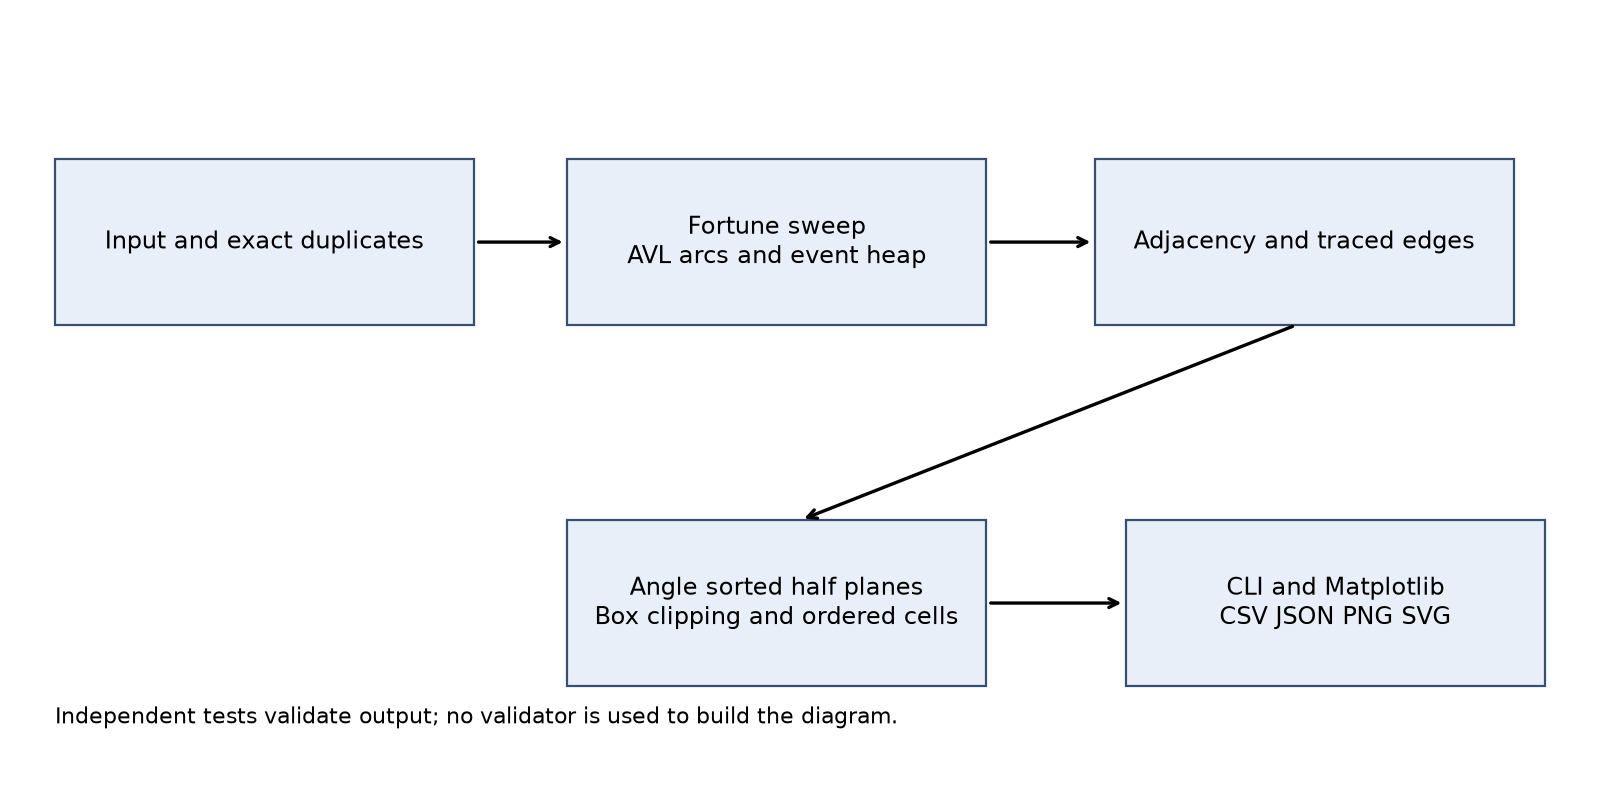
\includegraphics[width=1.0\linewidth,height=0.40\textheight,keepaspectratio]{architecture.png}
\caption{Construction pipeline and independent output validation.}
\label{fig:3}
\end{figure}

\begin{table}[!htbp]
\centering
\caption{Module responsibilities in the implemented system.}
\label{tab:2}
\begin{tabularx}{\linewidth}{@{}p{0.40\linewidth}X@{}}
\toprule
\textbf{Component} & \textbf{Main responsibility} \\
\midrule
\path{geometry.py} and \path{frame.py} & Filtered predicates, constructions and an exact uniform coordinate transform \\
\path{beachline.py} & Stable arc identities and AVL order \\
\path{events.py} and \path{circle.py} & Priority queue and candidate circle events \\
\path{sweep.py} & Site splits, arc removal, vertices and traced edges \\
\path{clipping.py} and \path{diagram.py} & Neighbour constraints and ordered clipped cells \\
\path{io.py}, \path{cli.py}, \path{interactive.py}, \path{visualize.py} & Inputs, exports, batch display and Delaunay overlay \\
\path{replay.py}, \path{replay_state.py}, \path{replay_canvas.py} & Event stepping, bounded checkpoints and browser replay \\
\bottomrule
\end{tabularx}
\end{table}

Each arc stores tree links, predecessor/successor links, height, site identifier, live state and a generation counter. A site can own several arcs, so its identifier cannot serve as a unique arc identity. Deletion transplants the successor node rather than copying its payload. This preserves queued references to the other arc objects.

\subsection{Invariants, Complexity and Numerical Policy}

The beach-line invariant is that the tree's in-order traversal equals the live left-to-right arc sequence, with consistent adjacent links. Search compares a query \(x\) against the node's current left and right breakpoints. AVL rotations preserve sequence order. Tests validate parent pointers, stored heights, balance and neighbour links after each randomized update.

The queue invariant is that the next valid event has the greatest remaining sweep height. The first heap key compares descending event heights. Ordinary separated heights use doubles; close circle heights are compared as exact rational-plus-square-root expressions. Event kind, horizontal position and a monotonically increasing serial number break equal-height ties. Site events precede circle events at equal height. A circle is valid only while its arc is alive and its stored generation equals the arc's current generation. Rescheduling increments that generation; stale entries are discarded when popped.

Each structural update creates only a constant number of candidates. AVL updates and heap operations cost $O(\log n)$, giving the intended $O(n \log n)$ sweep with $O(n)$ records. Traced adjacencies form a planar graph; hull order distinguishes true rays from zero-length cocircular diagonals. For cell degree \(k\), final intersection sorts \(k\) neighbour constraints plus four box constraints and uses a deque. Its cost is $O(k \log k)$; summing degrees in the planar graph preserves an $O(n \log n)$ overall target. It does not compare each cell with every site.

For neighbouring sites \(p_i\) and \(p_j\), the half-plane retained for \(p_i\) is equivalently
\begin{equation}
  2(p_j-p_i)\cdot q
  \leq \lVert p_j\rVert_2^2-\lVert p_i\rVert_2^2.
  \label{eq:halfplane}
\end{equation}
The implementation rescales this constraint and intersects only constraints generated by sweep neighbours.

\begin{table}[!htbp]
\centering
\caption{Numerical policies and their scope.}
\label{tab:3}
\begin{tabularx}{\linewidth}{@{}p{0.34\linewidth}X@{}}
\toprule
\textbf{Numerical operation} & \textbf{Current policy} \\
\midrule
Construction frame & Power-of-two scale with an exact translation or zero origin \\
Orientation cancellation & Filtered double sign, exact rational fallback \\
Close breakpoint searches & Exact rational comparison with the selected quadratic root \\
Ill-conditioned centre & Closest-pair origin and Decimal cancellation fallbacks \\
Close event heights & Exact comparison of rational radical expressions \\
Near-parallel half-planes & Rebuild coefficients from defining sites in Decimal \\
Clipping membership & Exact rational signs for uncertain corner tests \\
Repeated circle vertices & Exact input-circle identity, not coordinate rounding \\
\bottomrule
\end{tabularx}
\end{table}

These policies improved the tested cases, but they do not certify topology for every floating-point input. Coordinate construction still uses fixed 80-digit fallbacks and rounded output. A transform that loses subnormal coordinate bits is rejected explicitly. The complexity analysis counts arithmetic operations; the cost of exact rational fallbacks also depends on operand size. A fully certified geometry kernel would require stronger guarantees \cite{shewchuk1997}.

% Editable report section: Implementation and the AI-Assisted Coding Process
\section{Implementation and the AI-Assisted Coding Process}
\label{sec:4}

The site handler first locates the live arc above the new site. For an ordinary split it keeps the left arc identity, inserts the new site's arc and a right copy of the original site's arc, records their separating edge, then reschedules affected neighbours. Equal-height sites use an adjacent limiting arc instead of dividing by a zero directrix gap.

\begin{lstlisting}[caption={Local arc insertion during a site event.},label={lst:1}]
new, right = Arc(site), Arc(old.site)
self.beach.insert_after(old, new)
self.beach.insert_after(new, right)
self.edge(old.site, site)
for arc in (before, old, new, right, after):
    self.schedule(arc)
\end{lstlisting}

The circle handler verifies identity and generation before changing topology. It records the vertex on the two disappearing boundaries and on the newly created boundary, removes the middle arc and reschedules the surviving pair. These operations are local even though the output affects three cells.

\begin{lstlisting}[caption={Boundary updates during a valid circle event.},label={lst:2}]
self.edge(left.site, middle.site, vertex)
self.edge(middle.site, right.site, vertex)
self.edge(left.site, right.site, vertex)
self.beach.remove(middle)
self.statistics["circle_events"] += 1
self.schedule(left)
self.schedule(right)
\end{lstlisting}

AI-generated code was integrated incrementally: geometry passed ten tests, geometry plus AVL operations seventeen, and queue/circle examples twenty-one. The first complete cell suite then produced three genuine failures. Independent checks prompted corrections to clipping and numerical construction, documented in Section~\ref{sec:6}.

The snippets above are excerpts from the actual source. Complete editable modules and a companion source listing are included in the package. No public implementation was copied into the algorithmic core.

\subsection{Interfaces, Exports and Native Display}

The file parser accepts one whitespace- or comma-separated pair per line, ignores blank lines and comments, and reports malformed line numbers. Seeded generation uses Python's random generator. Exact duplicates retain their input-index groups. Batch commands print counts and construction timing, then optionally write an image, CSV and JSON.

\begin{figure}[!htbp]
\centering
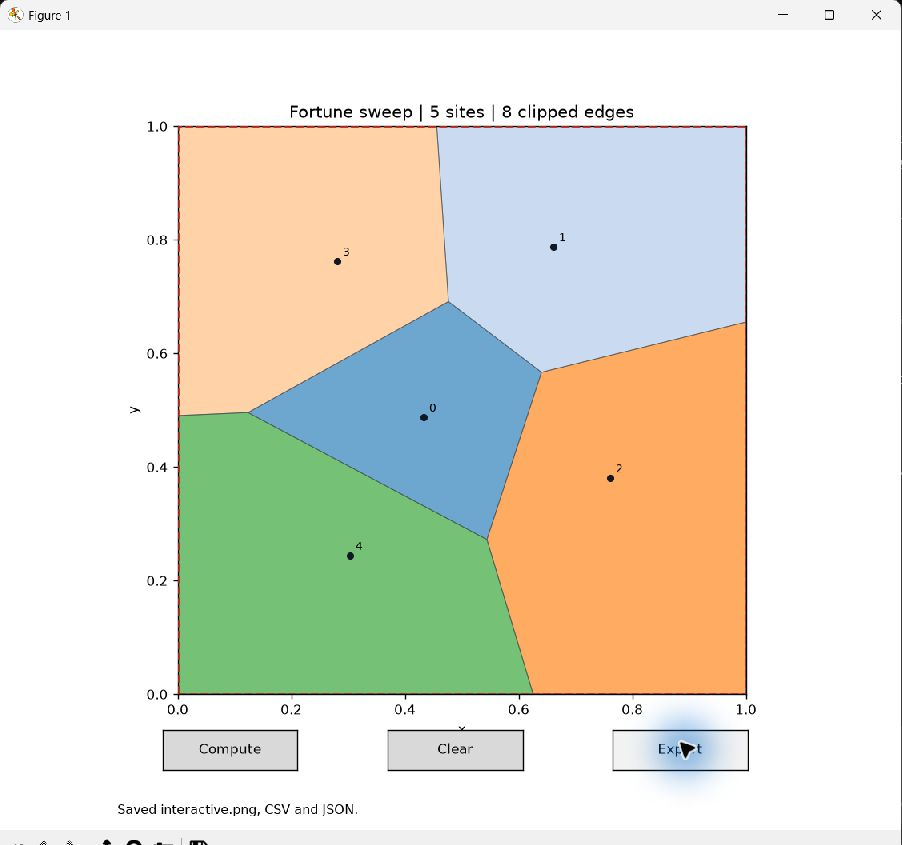
\includegraphics[width=0.92\linewidth,height=0.55\textheight,keepaspectratio]{gui-native.png}
\caption{Native Windows interface after a successful five-site export.}
\label{fig:4}
\end{figure}

The interface supports click insertion, Compute, Clear, Export and Animate. Callback tests exercise input and output; native Export produced PNG, CSV and JSON. Figure~\ref{fig:4} is a real capture of the earlier interface, before Animate was added. Its five-site state is retained in \path{examples/interactive.json}.

CSV rows give ordered vertices, next endpoints, neighbours and ray information. JSON includes defining sites and ray origins/directions. Static rendering supports an off-screen backend; interactive rendering needs a GUI backend \cite{matplotlibbackends}.

\subsection{Pointer-Controlled Sweep Replay}

Animate, or \code{--animate}, exports offline HTML. Python records live arc orders, queue previews, stale flags and edges from \code{FortuneSweep.step()}. Pointer movement selects a state by binary search; Canvas draws its parabolas as quadratic Bezier curves without rerunning Fortune. Play and Next event expose the same sequence. Appendix~\ref{sec:c} provides the capture and measurements.

The educational history can occupy $O(n^2)$ space and is capped at 200 distinct sites. It is excluded from ordinary $O(n\log n)$ construction benchmarks. The viewer explicitly identifies the production sorted-neighbour special case for collinear/minimal inputs.

% Editable report section: Testing and Validation
\clearpage
\section{Testing and Validation}
\label{sec:5}

The current suite passed all 171 tests on Windows with Python 3.14.7. The JUnit record is \path{data/current-tests.xml}. Its 16.62-second runtime includes validation and interface work, so it is separate from construction timing. Fixed seeds and retained inputs make the cases reproducible.

\begin{table}[!htbp]
\centering
\caption{Current automated validation results: 171 passing tests.}
\label{tab:4}
\begin{tabularx}{\linewidth}{@{}Xrc@{}}
\toprule
\textbf{Test family} & \textbf{Cases} & \textbf{Result} \\
\midrule
Geometry, singular limits and AVL structure & 18 & Pass \\
Queue and circle events & 4 & Pass \\
Random, degenerate, scale and invalid inputs & 42 & Pass \\
Tight clusters and high degree & 14 & Pass \\
Parser, exports, CLI and callbacks & 4 & Pass \\
Pi regression cases & 4 & Pass \\
Replay model, Canvas and Matplotlib inspector & 53 & Pass \\
Precision frame and close-event regressions & 12 & Pass \\
Delaunay overlay and interactive bounds & 11 & Pass \\
Independent reference comparison tests & 9 & Pass \\
\bottomrule
\end{tabularx}
\end{table}

Ownership validation first locates queries in the generated polygons and then compares their assigned sites with an independent linear nearest-site scan. Empty-circle checks compare defining-site distances and scan all sites for an interior point; clipping corners are excluded because they need not be circle centres. The precision regressions also use exact input-circle identities to check empty circles without a distance tolerance. Area totals and per-site positive-cell assertions complement the sampled queries.

The current stress check passed 300 seeded configurations of 10--89 sites and forty tight-cluster configurations. Separate 100-, 1,000- and 10,000-site cases each checked 100 ownership queries and every emitted vertex, including all 19,978 vertices in the largest case. The expanded precision campaign passed 800 deterministic uniform, jittered-grid, clustered and ring configurations, using 100 ownership queries per configuration. Their records are \path{data/current-stress.json} and \path{data/precision-validation.json}.

\clearpage
\subsection{Independent Reference Comparison}

The validation-only comparator uses SciPy 1.18.1 for Voronoi ridges and Delaunay triangles \cite{scipyvoronoi,scipydelaunay}. SciPy is pinned in \path{requirements-reference.txt} and is absent from the construction imports. A separate Sutherland--Hodgman clipper constructs reference cells against every site using exact rational inequalities. It shares neither the production sweep nor its angle-sorted half-plane intersection.

The default comparison covers 30 random seeds, three transformed datasets and twelve minimal, degenerate, duplicate or near-coincident inputs. Every case checks clipped-cell boundaries and areas against the exact validator, and sampled ownership against a SciPy nearest-neighbour query. For general-position cases, the Delaunay edge sets are also compared. Cocircular inputs may have different valid triangulation diagonals.

All 45 cases passed the geometric checks. SciPy fully resolved 39 cases. Five minimal or collinear inputs are outside its two-dimensional construction, and one near-cluster case loses a site under Qhull's precision handling. The exact validator covers those six cases; they are recorded separately rather than counted as SciPy matches. No input perturbation is used to turn them into reference successes.

For box span $s$ and maximum coordinate spacing $u$, boundary comparison uses $2\times10^{-8}s+16u$, and cell-area comparison uses $2\times10^{-8}s^2+32us$. The JSON record retains each input, seed, box, tolerance, library version, discrepancy list and reference limitation. An intentionally corrupted overlapping cell is detected by the comparator's own regression test. These checks support the tested cases within the stated tolerances, rather than certifying every floating-point configuration.

The complete result and its reproducible inputs are retained in \path{data/reference-comparison.json}.

\clearpage
\subsection{Degenerate Cases and Numerical Stress}

\begin{center}
\begin{minipage}{\linewidth}
\captionsetup{hypcap=false}
\centering
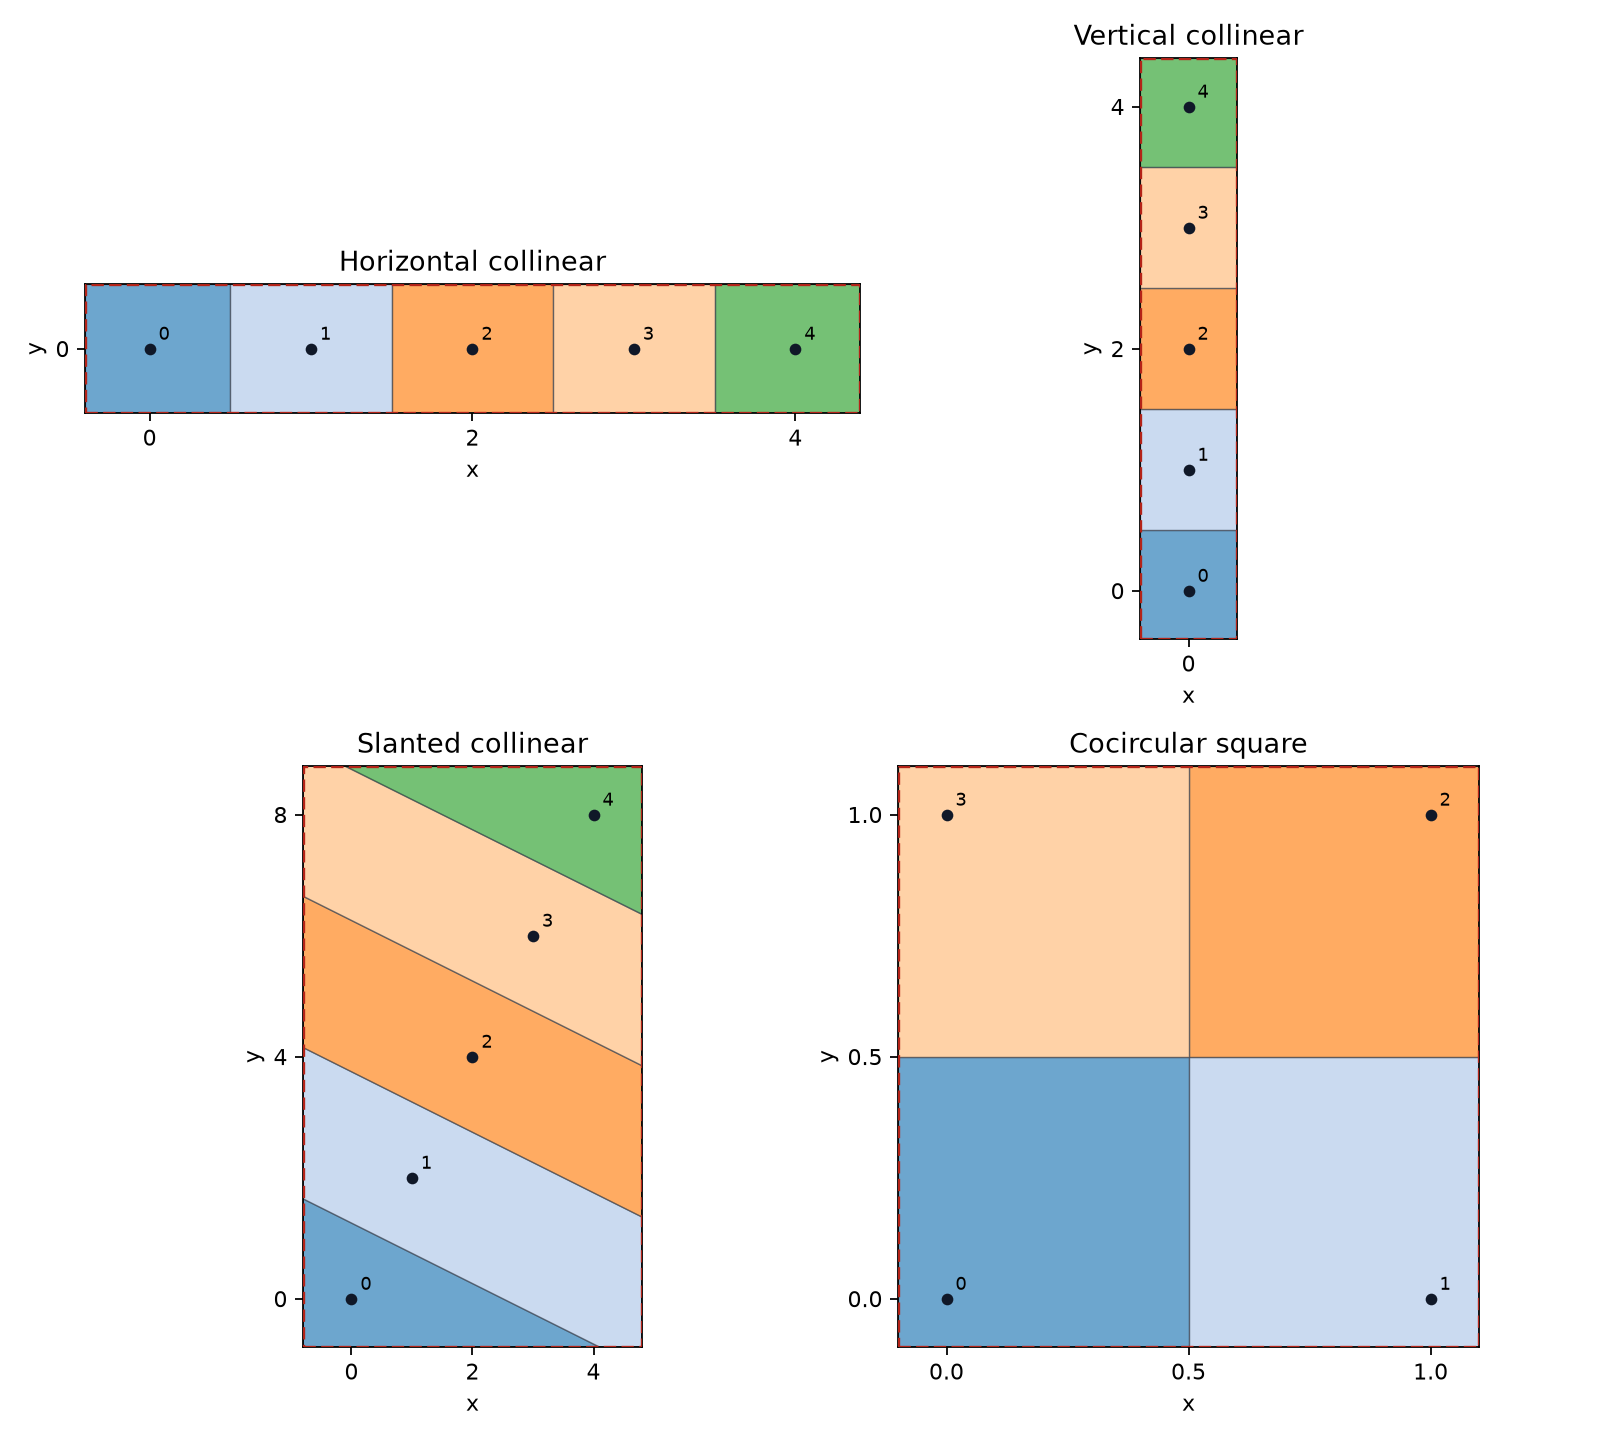
\includegraphics[width=1.0\linewidth,height=0.65\textheight,keepaspectratio]{degenerate-1.png}
\captionof{figure}{Horizontal, vertical and slanted collinear inputs, and a cocircular square.}
\label{fig:5}
\end{minipage}
\end{center}

The three line directions give parallel bisector strips. The square produces one common circle vertex; a zero-length diagonal is not drawn as a real edge.

\clearpage
\subsection{Duplicate, Nearly Coincident and Minimal Inputs}

\begin{center}
\begin{minipage}{\linewidth}
\captionsetup{hypcap=false}
\centering
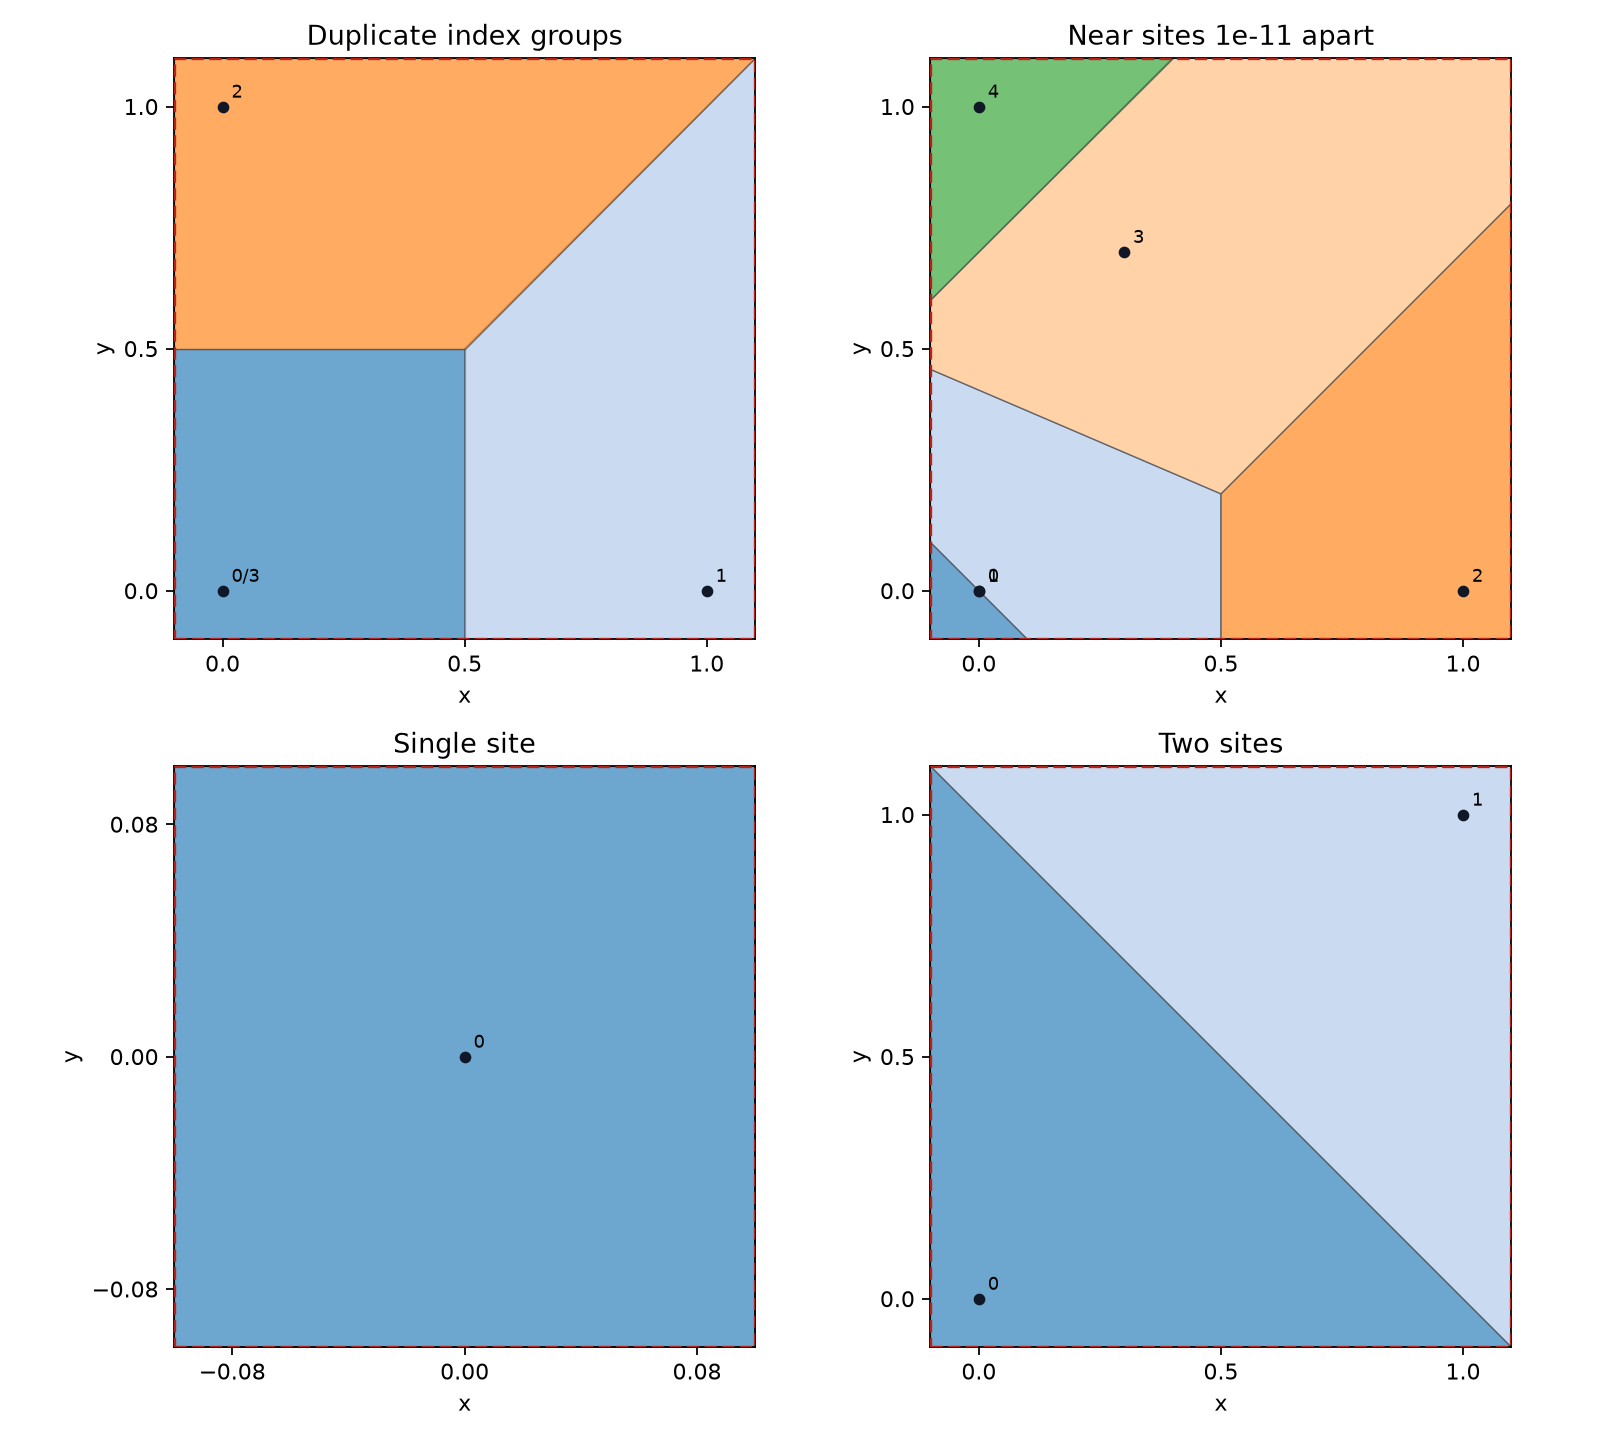
\includegraphics[width=1.0\linewidth,height=0.65\textheight,keepaspectratio]{degenerate-2.png}
\captionof{figure}{Duplicate, nearly coincident, single-site and two-site inputs.}
\label{fig:6}
\end{minipage}
\end{center}

Indices \code{0/3} in the duplicate example share one cell. In the near-site panel, sites separated by $10^{-11}$ are distinct but cannot be visually resolved at the full plot scale. Automated checks, rather than marker separation, establish their treatment. The adversarial tests additionally place six sites within clusters down to $10^{-15}$ among distant sites. Passing these cases under stated tolerances does not certify every near-degenerate input.


The numerical checks use tolerances that account for both construction error and the spacing of exported world coordinates. Passing a selected tight-cluster input therefore supports that case within its stated tolerances; it does not establish correctness for every possible floating-point input. Exact duplicates are grouped deliberately. The constructor rejects a coordinate range if its normalization loses subnormal bits.

\clearpage
% Editable report section: Problems and Solutions
\section{Problems and Solutions}
\label{sec:6}

\subsection{Rounded Zero-Length Edges}

\textbf{Symptom.} The diagonal two-site and nine-site cocircular examples reported holes during cell-ownership sampling, while their total-area checks passed.

\textbf{Investigation.} Consecutive polygon endpoints and their cross products were inspected. Three concurrent constraints had created nearly equal output vertices and a tiny boundary segment.

\textbf{Root cause.} Subtracting rounded equal endpoints gave an arbitrary segment direction. The convex-containment check then treated that segment as an additional, incorrect boundary constraint.

\textbf{Solution.} The final cleanup removes a support only when \code{concurrent(p,q,r)} proves exact rational concurrence. An intermediate distance cutoff was rejected after per-site checks found missing tiny cells. Exact circle identities also replace rounded-centre grouping.

\textbf{Verification.} The original failures and six new positive-cell regressions pass. The later failing cases are retained in \path{tiny-cell-initial.xml}.

\textbf{Prevention and lesson.} Check that every site retains its cell; area and sampled ownership alone can miss microscopic missing cells.

\subsection{Close-Site Half-Plane Coefficients}
\label{prob:coefficients}

\textbf{Symptom.} A seed-11 cluster at scale $10^{-11}$ produced area 1.439996905390856 for a box of area 1.44.

\textbf{Investigation.} Cluster inputs and polygon intersections were compared with ordinary random cases. The problem appeared when almost parallel bisectors were intersected.

\textbf{Root cause.} Unit-normal coefficients had already lost precision before division by a small intersection determinant. More precision applied only to those rounded coefficients could not recover the missing information.

\textbf{Solution.} \code{HalfPlane} retains its defining focus pair. For \code{abs(det) < 1e-7}, coefficients are rebuilt from those binary coordinates and intersected using 80-digit Decimal arithmetic.

\textbf{Verification.} The seed-11 cluster now passes area, ownership and empty-circle checks.

\textbf{Prevention and lesson.} Preserve construction provenance and identify the conditioning of arithmetic operations, not just the final output's finiteness.

\subsection{Predicate Reliability versus Construction Accuracy}

\textbf{Symptom.} The initial exponent-15 cluster emitted a centre that failed equidistance to its defining sites. The original failure and input are saved in \path{adversarial-initial.json}.

\textbf{Investigation.} The determinant used for the centre was compared with its product magnitudes. Its sign was plausible, but the calculated coordinates remained inaccurate.

\textbf{Root cause.} The original relative fallback threshold of \(8\times 10^{-16}\) addressed severe sign cancellation. A sign filter does not provide an accuracy guarantee for the division used to construct a circumcentre.

\textbf{Solution.} With translated vectors \(u=b-a\) and \(v=c-a\), the circumcentre is recomputed in Decimal when
\begin{equation}
  \lvert u_xv_y-u_yv_x\rvert
  \leq 10^{-8}\bigl(\lvert u_xv_y\rvert+\lvert u_yv_x\rvert\bigr).
  \label{eq:centre-filter}
\end{equation}
This construction policy is separate from the orientation predicate.

\textbf{Verification.} All five tight-cluster exponents pass the circle tests.

\textbf{Prevention and lesson.} Distinguish decisions about a determinant's sign from coordinate construction. The AI's first implementation conflated the two, and adversarial tests exposed the gap.

\subsection{A Generous Epsilon Created Invalid Boundary Edges}
\label{prob:epsilon}

\textbf{Symptom.} After the precision changes, exponent-13 and exponent-14 clusters still reported a hole at \((0.783765456996815,\,0.7120393849074937)\).

\textbf{Investigation.} A corner cell contained a vertex at \(y=1.100000000000123\) despite a clipping maximum of \(1.1\). A reversed edge about \(1.2\times 10^{-13}\) long excluded valid interior queries.

\textbf{Root cause.} The original membership allowance of \(2\times 10^{-13}\) kept an inactive constraint and admitted a corner just outside the rectangle. Relaxing the validator did not repair that polygon.

\textbf{Solution.} The first fix reduced the allowance to \(8\times 10^{-16}\); final \code{corner\_inside} uses exact rational signs when the floating result is uncertain.

\textbf{Verification.} The two failures saved in \path{tests-adversarial.xml} pass afterward.

\textbf{Prevention and lesson.} Increasing epsilon is not a universal repair; construction must be rechecked against independent geometric properties.

\subsection{A Validator Omitted Output Representation Error}

\textbf{Symptom.} Translating an otherwise small input near \(10^9\) caused an equidistance failure under the original fixed $10^{-8}$ validation allowance.

\textbf{Investigation.} The spacing between representable output coordinates was measured. One double-precision ULP near \(10^9\) is about \(1.19\times 10^{-7}\), already larger than that validation bound. The constructor calculates locally but must round when it returns world coordinates.

\textbf{Root cause.} The validator assumed that normalization eliminated all scale effects, including final coordinate representation. It also underestimated cross-product uncertainty for extremely short exported edges.

\textbf{Solution.} The circle-distance tolerance is
\begin{equation}
  \tau_{\mathrm{circle}}
  =10^{-8}\max(1,r)+8\,\operatorname{ulp}_{\mathrm{world}},
  \label{eq:validation-tolerance}
\end{equation}
where \(\operatorname{ulp}_{\mathrm{world}}\) is the float spacing at the largest absolute vertex coordinate. Polygon containment also includes endpoint-subtraction uncertainty and a bounding-box rejection. These bounds describe representation error; they do not replace the ownership check with a direct site scan.

\textbf{Verification.} The translation and scaling cases pass. Cluster tests still failed until the distinct construction defects in Sections~\ref{prob:coefficients}--\ref{prob:epsilon} were fixed, showing that the validator change alone did not hide those defects.

\textbf{Prevention and lesson.} A validator is software with its own assumptions. Review its error model and preserve independent checks that can disagree with it. A passing tolerance-based test is evidence within a stated precision regime, not a universal proof.

The five cases above were observed during actual development. Their symptoms, inputs, fixes and regression checks are retained in \path{docs/problems.md} and \path{evidence/}. Additional environment issues included pip bootstrapping into an unwritable temporary directory and a duplicate dictionary key in the first benchmark script. Those were corrected and are recorded as engineering issues rather than substituted for the five geometric analyses.

\clearpage
% Editable report section: Performance Analysis and Results
\section{Performance Analysis and Results}
\label{sec:7}

Benchmarks used Windows 11 x64, Python 3.14.7 and an Intel64 Family 6 Model 165 processor. Each size used seed 2026 and the unit-square box. Table~\ref{tab:5} reports the median of three uninstrumented timing runs and separate memory measurements. Construction includes deduplication, normalization, the sweep, clipping and cell assembly; input generation, validation, plotting and export are excluded.

\begin{table}[!htbp]
\centering
\caption{Measured performance for seeded construction workloads.}
\label{tab:5}
\begin{tabularx}{\linewidth}{@{}rXXX@{}}
\toprule
\textbf{Sites} & \textbf{Median seconds} & \textbf{Python peak MiB} & \textbf{Process peak MiB} \\
\midrule
100 & 0.03294 & 0.70 & 23.67 \\
1,000 & 0.40641 & 7.38 & 41.42 \\
10,000 & 4.35665 & 65.08 & 217.48 \\
\bottomrule
\end{tabularx}
\end{table}

\begin{figure}[!htbp]
\centering
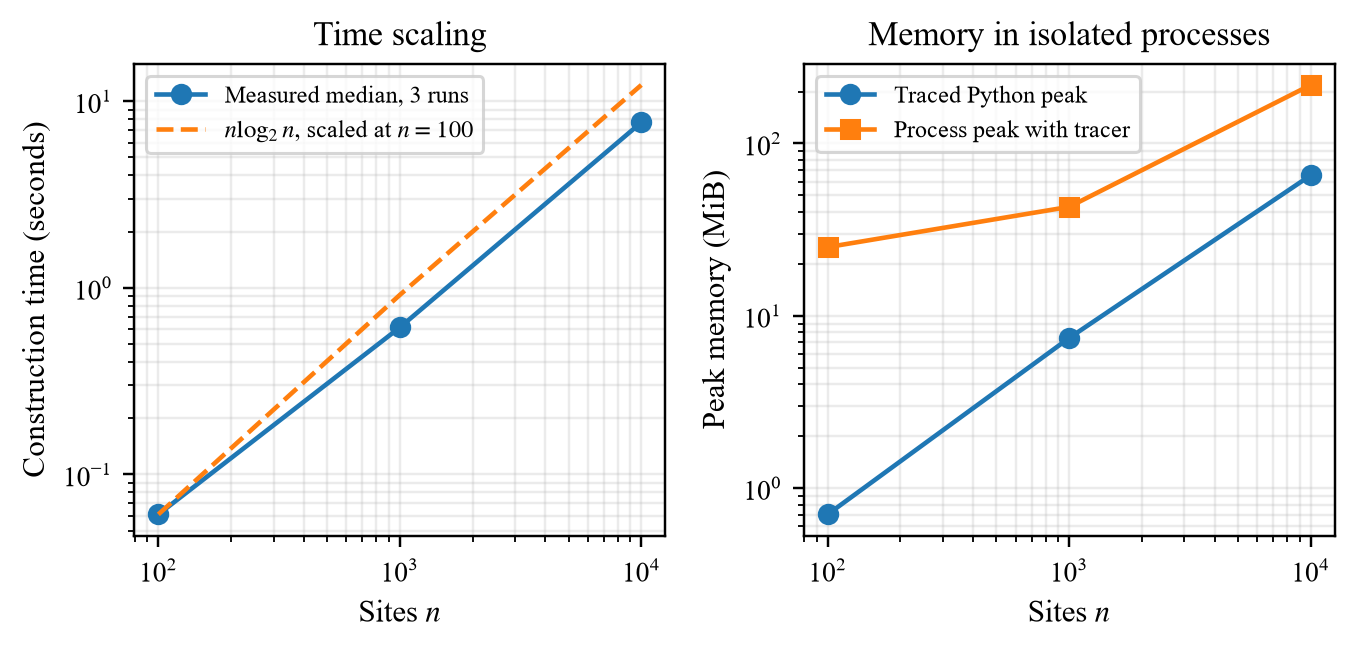
\includegraphics[width=1.0\linewidth,height=0.43\textheight,keepaspectratio]{scaling.png}
\caption{Measured construction time and isolated-process memory peaks.}
\label{fig:7}
\end{figure}

Memory was measured in fresh processes. Tracemalloc started after input generation and recorded Python allocations during construction. Process peak working set included the interpreter, input and instrumentation; it therefore does not measure uninstrumented incremental algorithmic memory \cite{pythontracemalloc}.

Tenfold input increases yielded time ratios of approximately 12.34 and 10.72. Python allocation peaks grew approximately tenfold. These observations are consistent with the intended \(O(n\log n)\) time and \(O(n)\) space, but three sizes do not prove asymptotic bounds. Full platform metadata, scope and per-run values are preserved in \path{results/benchmark.json}.

\clearpage
% Editable report section: Critical Reflection on AI-Assisted Programming
\section{Critical Reflection on AI-Assisted Programming}
\label{sec:8}

The most difficult part of the project for me was understanding the concept of Fortune's algorithm. AI could help produce code, but I still needed to understand the geometric idea behind it. Online explanations were useful in this process. In particular, Jacques Heunis's intuitive explanation made the concept easier for me to understand~\cite{heunis2018}. I used it as a conceptual learning resource.

AI was helpful in translating the basic concept into Python code and implementing the Fortune sweep, including event handling and the beach line. Debugging still required active checking. My workflow included inspecting outputs and using Pi to edit code and rerun tests. Generated code was therefore part of a cycle of inspection, correction and rechecking. I should be able to explain the resulting implementation, rather than treating the tool's response as sufficient evidence of correctness.

A correct-looking diagram was not enough to give me confidence in the result. Checking the CSV export and running tests added evidence beyond the picture. During my review, I confirmed that an exported cell boundary closed and personally ran the suite that reported 82 passing tests. The expanded suite includes four Pi-generated regressions. I also supplied genuine captures of Pi reviewing the invariants and tiny-cell correction, and rerunning the suite: 86 tests passed in 7.09 seconds. This is separate from the desktop assistant's 5.43-second run.

AI-generated documentation also needed review. The initial report did not meet my expectations for presentation, so I requested LaTeX source, properly typeset mathematics and clearer code formatting. This was a concrete example of why detailed requirements and review remained necessary even when the tool had produced a complete-looking document.

The development records show more serious limits in generated numerical code. A reliable orientation sign did not ensure an accurate circumcentre, and sampled checks missed microscopic cells. Those failures required independent geometric checks and specific regression inputs. Prompts tied to an invariant, failing input and expected behaviour were more useful than broad requests for robust geometry. Both AI tools used the GPT-6.1 family, so using Pi did not provide an independent correctness oracle.

My overall takeaway is that AI helped turn the concept into an implementation, while learning, debugging and verification remained essential. Further work should strengthen precision-limit tests and independent validation. The narrated demonstration is also important: it requires me to explain the architecture, invariants and numerical decisions in my own words.

\clearpage
% Editable report section: Conclusion
\section{Conclusion}
\label{sec:9}

The project now contains a working, from-scratch Fortune sweep with an AVL beach line, event invalidation, traced edges and clipped ordered cells. It provides reproducible input modes, machine-readable exports, static visualization and a native interactive window. Eighty-six automated tests and additional seeded checks pass. Actual benchmarks reach 10,000 sites with time and allocation growth consistent with the intended $O(n \log n)$ and $O(n)$ targets.

The principal limitations are finite-precision topology beyond the tested regimes, the absence of external reference cross-validation and the need for broader platform verification. Windows 11 was exercised; Windows 10 compatibility is a target, not a tested claim. Genuine AI interaction screenshots and the owner's reflection are included. The remaining personal tasks are the narrated walkthrough and final review of the report and package.

The software and report are designed to be explained as well as run. The strongest contribution is the combination of a genuine sweep implementation with independent checks and retained failure evidence. The final demonstration should focus on those mechanisms and their practical limits.


\clearpage
\phantomsection
\addcontentsline{toc}{section}{References}
\bibliographystyle{ieeetr}
\bibliography{references}
\label{last-main-page}

\clearpage
\appendix
% Appendix A is supplied in source_appendix.pdf; B--D remain in this volume.
\setcounter{section}{1}
% Development record condensed from the retained technical entries.
\section{Development Record}
\label{sec:b}

The development record tracks the construction of the program, the failures that changed it, and the checks used before accepting each stage. The earlier technical entries are dated 10 November 2026, while the current verification is summarized at the end of this appendix. That record is retained in \path{data/development-record.txt}, with the test and measurement records under \path{data/}.

\subsection{Git Commit History}

Table~\ref{tab:git-history} summarizes the local repository's recorded commits. Dates are shown in GMT+8. The source snapshot also contains the current implementation changes covered by the November 18 verification.

\begingroup
\setstretch{1.05}
\renewcommand{\arraystretch}{1.08}
\begin{longtable}{@{}p{0.19\linewidth}p{0.77\linewidth}@{}}
\caption{Recorded Git commit dates and implementation stages.}\label{tab:git-history}\\
\toprule
\textbf{Commit date} & \textbf{Recorded changes} \\
\midrule
\endfirsthead
\toprule
\textbf{Commit date} & \textbf{Recorded changes} \\
\midrule
\endhead
\bottomrule
\endfoot
24 Oct 2026 & Requirements, architecture and development records. \\
25 Oct 2026 & Stable geometry primitives and initial unit tests. \\
26 Oct 2026 & AVL beach line with stable arc identities and neighbour links. \\
27 Oct 2026 & Deterministic sweep-event priority queue. \\
28 Oct 2026 & Clockwise circle-event detection and stable event heights. \\
30 Oct 2026 & Site splits, circle-event processing and traced sweep edges. \\
1 Nov 2026 & Clipped ordered cells and degenerate-case validation. \\
3 Nov 2026 & Ill-conditioned geometry and clipping-tolerance corrections. \\
5 Nov 2026 & Text input, seeded generation, batch commands and ray exports. \\
6 Nov 2026 & Coloured diagrams and interactive Compute and Export controls. \\
7 Nov 2026 & Construction-time and memory measurements, with reproducible figures. \\
8 Nov 2026 & Clean-installation checks, extended stress tests and Windows/Linux CI. \\
8 Nov 2026 & Microscopic cells and exact circle identities. \\
8 Nov 2026 & Tiny-cell and cocircular-ray corrections with stricter regressions. \\
9 Nov 2026 & Verified figures and walkthrough materials. \\
10 Nov 2026 & Cross-platform checks and extracted-package verification. \\
11 Nov 2026 & Stepwise Fortune replay and retained project evidence. \\
12 Nov 2026 & Pointer-following Canvas replay and inspector controls. \\
14 Nov 2026 & Integrated pointer replay and verification checks. \\
14 Nov 2026 & Main-branch CI results and delivery checks. \\
14 Nov 2026 & Archive checksum records. \\
\end{longtable}
\endgroup



\subsection{Requirements and Architecture}

The initial checklist covered input, output, validation and delivery. The selected architecture used an AVL beach line, a heap event queue and validators separate from construction.

\subsection{Geometry and Sweep Construction}

Geometry initially passed ten tests; adding the beach line raised this to seventeen, and sweep integration to twenty-one. Seeded AVL updates checked parent pointers, balance and neighbour order. Triangle and simultaneous-circle cases checked event processing.

\subsection{Cell Construction and Numerical Corrections}

The first complete cell suite had 59 passes and three failures. Corrections to rounded zero-length edges and output-coordinate tolerances produced 62 passes. Tight clusters exposed the further conditioning and membership problems discussed in Section~\ref{sec:6}. Per-site checks then exposed missing microscopic cells. Exact concurrence and input-circle identities preserved their topology, bringing the earlier suite to 82 tests.

\subsection{Stress Tests and Measurements}

The earlier campaign checked 300 random and forty clustered configurations, plus every vertex in the large cases. The separate November 10 benchmark used three construction timings per size; a new November 18 run repeats the procedure for the current engine. An exact twelve-site integer circle also exposed redundant diagonals: hull adjacency separated its twelve rays from zero-length edges, leaving one central vertex.

\subsection{Clean Installation and Delivery Checks}

Earlier clean-environment checks verified import, the 82-test suite and PNG, CSV and JSON exports. Their original records remain under the core filenames in \path{data/}.

\subsection{Replay and Current Verification}

Shared event stepping, seek checkpoints, Canvas replay and a Matplotlib inspector extended the implementation. Pi contributed four retained regressions; replay and interface coverage brought the suite to 139 tests. Precision, Delaunay and reference checks bring the current total to 171.

Current verification passed 800 precision configurations and repeated the random/cluster stress campaign, including all 19,978 vertices at 10,000 sites. All 45 reference datasets passed exact clipped-cell checks, with 39 complete SciPy comparisons and six recorded reference limitations. The source archive matches the implementation associated with these results.

\clearpage
% Actual viewer capture and separately measured renderer diagnostics.
\section{Sweep Replay and Rendering Evidence}
\label{sec:c}

\begin{figure}[!htbp]
\centering
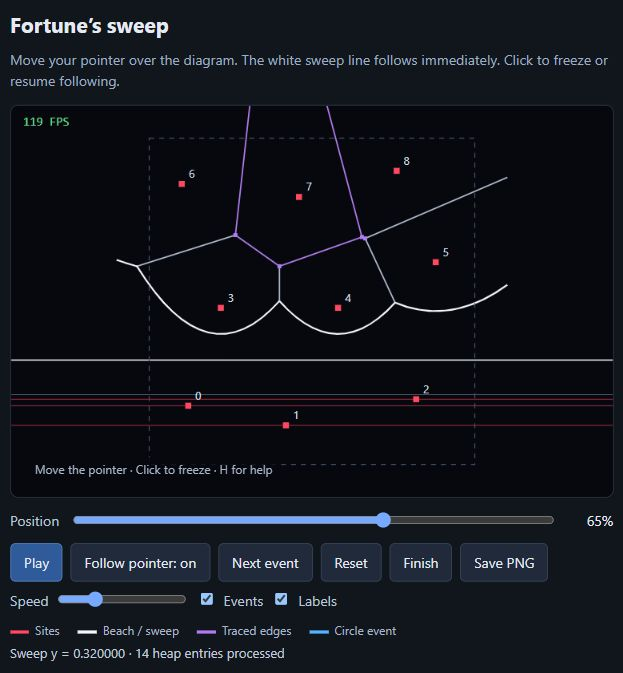
\includegraphics[width=0.83\linewidth,height=0.62\textheight,keepaspectratio]{canvas-preview.jpg}
\caption[Pointer-controlled Canvas sweep replay.]{Actual browser capture of the integrated viewer. Red squares are sites; white curves and the horizontal line are the beach line and directrix. Purple segments are traced edges. Event markers and controls expose the recorded Python event sequence.}
\label{fig:canvas-replay}
\end{figure}

Run \code{run.bat --animate --input examples\textbackslash sites.txt}. Hover to move the sweep line, click to freeze or resume following, or use Play and Next event. The exported HTML works offline. \path{docs/animation.md} describes controls, the collinear special case and the history limit.

\clearpage
\subsection{Rendering Bottleneck and Verification}

The first Matplotlib replay rebuilt axes, artists and interface text on every frame. A 50-site off-screen redraw took a median 234.36 ms, while event-model advancement took about 0.007 ms. Persistent artists, background caching and time-based playback improved the native Tk version to about 44.5 timer updates per second. The owner still found pointer interaction insufficiently fluid. The final viewer therefore records event facts once and draws them directly in browser Canvas.

\begin{table}[!htbp]
\centering
\caption{Observed browser rendering diagnostics, separate from construction.}
\label{tab:canvas-performance}
\begin{tabularx}{\linewidth}{@{}rXX@{}}
\toprule
\textbf{Sites} & \textbf{Rolling RAF rate} & \textbf{Median draw time} \\
\midrule
50 & 120.0 Hz & 1.4 ms \\
200 & 120.0 Hz & 2.4 ms \\
\bottomrule
\end{tabularx}
\end{table}

Measurements came from the visible in-app browser at 602 by 375 CSS pixels, with a 752 by 469 backing canvas. The rate measures rolling \code{requestAnimationFrame} callbacks, not physical display scanout; draw time covers recent Canvas work. These observations do not guarantee a frame rate on other displays or machines. Browser console checks reported no errors. Position changes, playback and Save PNG were exercised; the original downloaded image is \path{evidence/canvas-export.png}. Raw diagnostics are retained in \path{results/animation-preview/render-browser.json}.

The revised viewer uses the same Python event handlers as batch construction, but its stored arc orders can occupy $O(n^2)$ space. A 200-site limit keeps this educational trade-off explicit. Core construction creates no replay history. The owner approved the viewer's appearance and authorized main-branch integration on 18 November 2026. That approval does not substitute for the owner's narrated explanation of the algorithm.

Replay tests compare every snapshot with a separately run Python sweep and verify independent checkpoints. Two Node-based checks compare drawing geometry with Python in 100 cases and exercise pointer movement without a pressed button; they explicitly skip without Node. Installed-asset and browser checks cover offline export, positioning, playback and PNG download. Node is unnecessary to run the viewer.

\clearpage
% Original prompt-and-response captures, explained in Section 2.
\section{AI Interaction Evidence}
\label{sec:d}

The first interaction concerns the beach-line and event-queue invariants. Its response explains why rotations preserve arc order and why generation counters invalidate obsolete circle predictions. The guard is checked by the retained stale-event regressions.

\begin{figure}[!htbp]
\centering
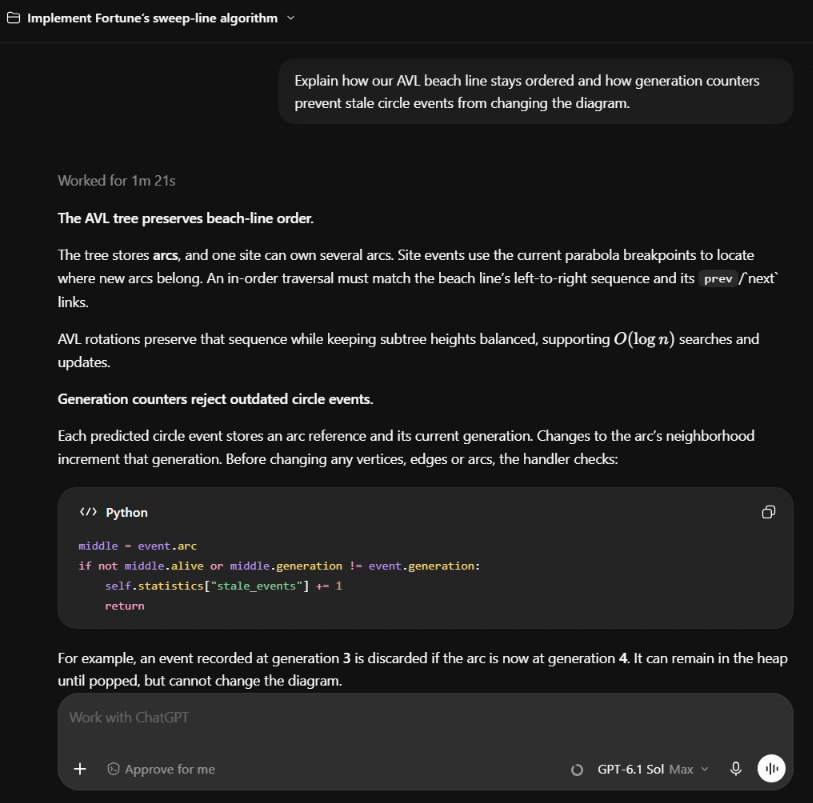
\includegraphics[width=0.99\linewidth,height=0.73\textheight,keepaspectratio]{ai-interaction-1.png}
\caption{ChatGPT prompt and response explaining AVL order and stale circle-event rejection.}
\label{fig:ai-chatgpt}
\end{figure}

\clearpage
\begin{landscape}
\thispagestyle{empty}
\captionsetup{hypcap=false}
\centering
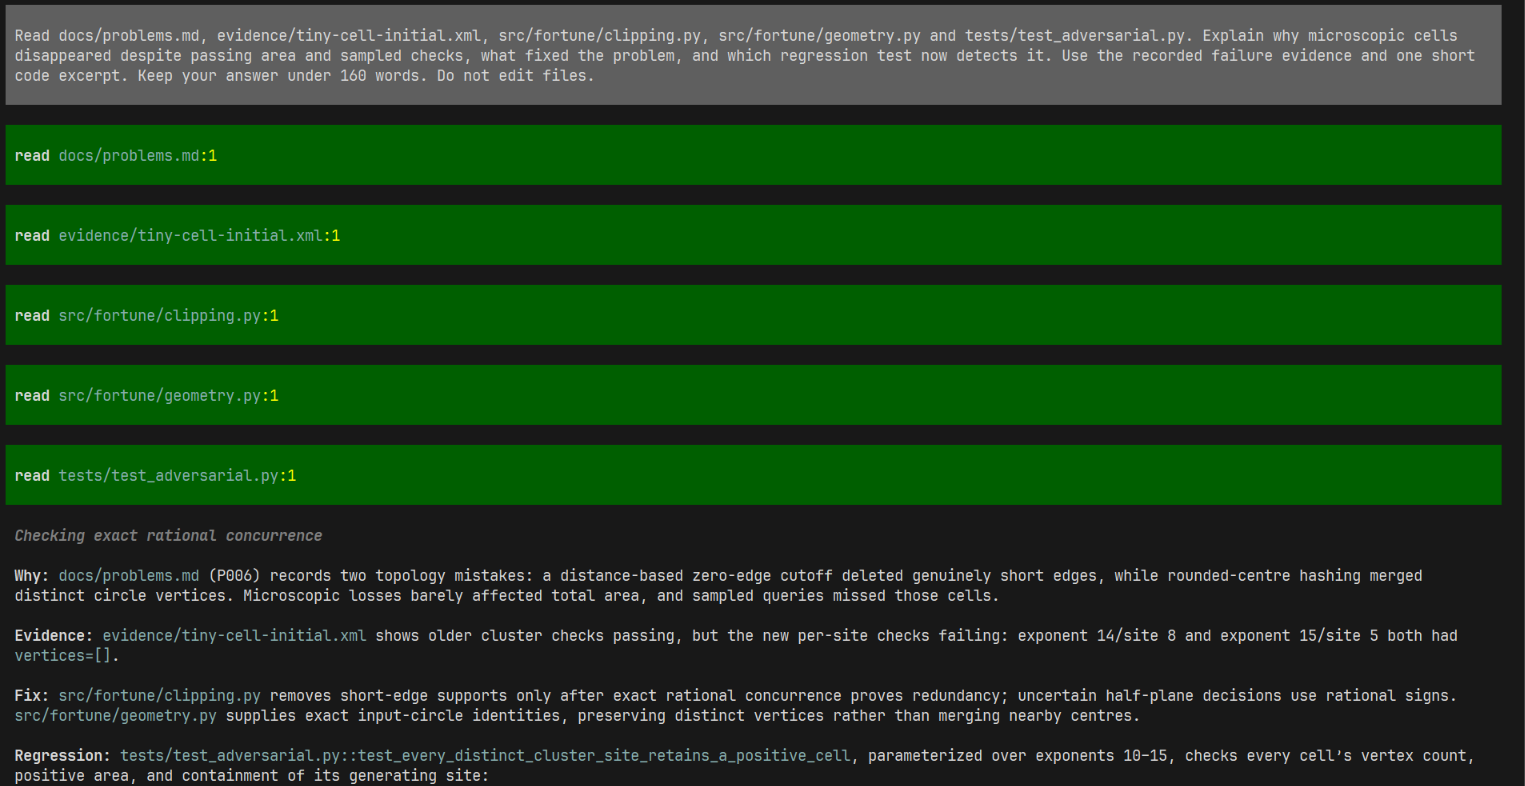
\includegraphics[width=\linewidth,height=116mm,keepaspectratio]{ai-interaction-2.png}\par
\vspace{2mm}
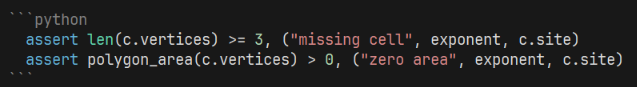
\includegraphics[width=115mm,height=16mm,keepaspectratio]{pi-tiny-cell-code-continuation.png}\par
\captionof{figure}{Pi prompt and response investigating microscopic cells, followed by the per-site regression excerpt.}
\label{fig:ai-pi}
\vspace{2mm}
{\fontsize{10}{12}\selectfont\thepage\par}
\end{landscape}

\end{document}
